\textbf{Seats}
\begin{enumerate}
    \item 5 mins: Intro slides \par
    \item 20 mins: Finish Example 6.2.1 \par
    \textbf{Check piazza}
    \item 35 mins: Finish Example 6.3.1 \par
    \textbf{Check piazza}
    \item 50 mins: Finish Example 6.3.2 \par
    \textbf{Check piazza}
\end{enumerate}
\textbf{Seats}

\textbf{Example 6.2.1}

To draw the solution
\begin{itemize}
\item Find the stationary points. ${\rm d}y/{\rm d} x = 0$ when $x+y=0$ so $y=-x$. So draw horizontal arrows along the line $y=-x$.
\item The gradient increases as both $x$ and $y$ increase, so draw arrows pointing down and to the right below/left of $y=-x$ and pointing up and to the right above/right of $y=-x$.
\item Note that at $y = -x - 1$ the arrows have gradient $-1$, so they will carry on parallel to the stationary point. (Students wouldn't be expected to find this unaided in an exam). 
\item Draw solutions starting at various points from $x=0$. If we choose $y<-1$ we see the solution just keeps decreasing. For $y=-1$ it runs parallel to the stationary point. For $-1 < y < 0$ the line begins decreasing and crosses the line $y=-x$ to end up increasing. For $x>0$ the solution is always increasing.
\end{itemize}

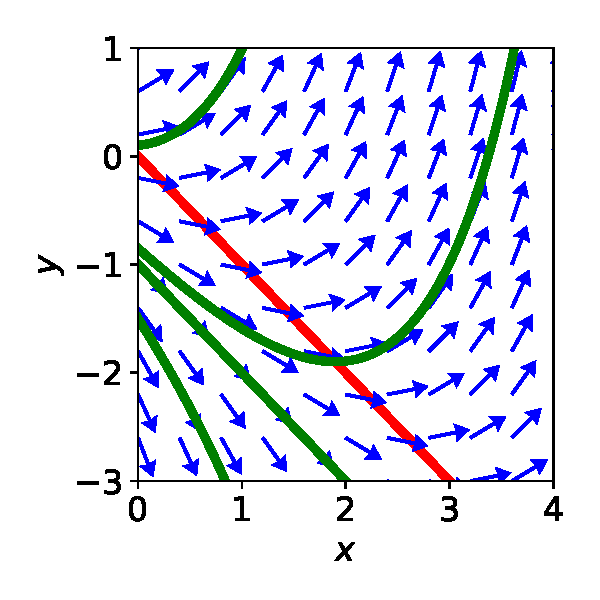
\includegraphics{Figures/ex_621.pdf}

\vspace{10mm}
\textbf{Example 6.3.1}

\begin{align*}
\frac{{\rm d} y}{{\rm d} x} = \frac{y}{x} 
\end{align*}
which separates to
\begin{align*}
\int \frac{1}{y} \, {\rm d} y = \int \frac{1}{x} \, {\rm d} x 
\end{align*}
Integrating gives
\begin{align*}
\ln|y| &= \ln|x| + c \\
|y| &= e^{\ln|x| + c} = Ae^{\ln|x|} = A|x|
\end{align*}
for $A > 0$. Therefore $y = Bx$ where $B = \pm A$ and since $y=2$ when $x=1$ we have $A=2$.  Therefore the particular solution is 
\begin{align*}
y = 2x \, .
\end{align*}

\vspace{10mm}
\textbf{Example 6.3.2}

I'm going to start by taking a factor of $-1$ out of the RHS, so this looks more like the partial fractions we're used to. 
\begin{align*}
\frac{{\rm d} y}{{\rm d} t} = - y(y-1)
\end{align*}
which separates to
\begin{align*}
\int \frac{1}{y(y-1)} \, {\rm d} y = \int (-1) \, {\rm d} x 
\end{align*}
The integrand on the LHS can be separated using partial fractions
\begin{align*}
\frac{1}{y(y-1)} &= \frac{A}{y} + \frac{B}{y-1}\\
1 &= A(y-1) + By
\end{align*}
Setting $y=0$ gives $A=-1$ and setting $y=1$ gives $B=1$. Therefore the integral becomes
\begin{align*}
\int \left(-\frac{1}{y} + \frac{1}{1-y}\right) \, {\rm d} y = \int (-1) \, {\rm d} x \\
-\ln|y| + \ln|y-1| &= -x + c \\
\ln\left(\left| \frac{y-1}{y} \right|\right) &= -x + c \\
\left| \frac{y-1}{y} \right| &= Ae^{-x} \, ,
\end{align*}
for some positive $A$. Defining a new constant $B = \pm A$ we can write
\begin{align*}
\frac{y-1}{y} &= Be^{-x} \\
1 - \frac{1}{y} &= Be^{-x} \\
 \frac{1}{y} = 1 -  Be^{-x} \\
 y = \frac{1}{1 - Be^{-x}} \\
 y = \frac{e^x}{e^{x} - B} \\
\end{align*}
Now, when $x=0$ we have $B = (y-1)/y$, so if the initial condition is
\begin{itemize}
\item $y= -0.01$, then $(-1.01)/(-0.01) = 101$, so the p.s. is $y = e^x/(e^x - 101)$, which is negative and decreasing until $e^x > 101$ at which point it switches sign and heads towards $y = 1$.
\item $y= 0.01$, then $(-0.99)/(0.01) = -99$, so the p.s. is $y = e^x/(e^x + 99)$, which is positive and increasing but bounded at $y = 1$ as the numerator cannot be larger than the denominator.
\item $y = 0.5$, then  $(-0.5)/(0.5) = -1$, so the p.s. is $y = e^x/(e^x + 1)$, which is positive and increasing but bounded at $y = 1$ as the numerator cannot be larger than the denominator.
\item $y = 2$, then  $(1)/(2) = 1/2$, so the p.s. is $y = e^x/(e^x - 1/2)$, which is positive but decreasing and bounded at $y = 1$ as the denominator cannot become larger than the numerator.
\end{itemize}
